\section{RL for RAG Agent}

% \textcolor{violet}{Mark: writing from first principles perspective; from a basic starting point and then draw the connection to the VPG.}

% \textcolor{violet}{Mark: emphasize the technical challenges.}
% By Muzhi, 这里大标题是否要这么写需要考虑一下，因为我们有个第一阶段的SFT。当然除非说第一阶段的SFT不写了，或者我们写成 “手动RL” （这有点整活儿(搞嘢)了）..

\begin{figure*}
    \centering
    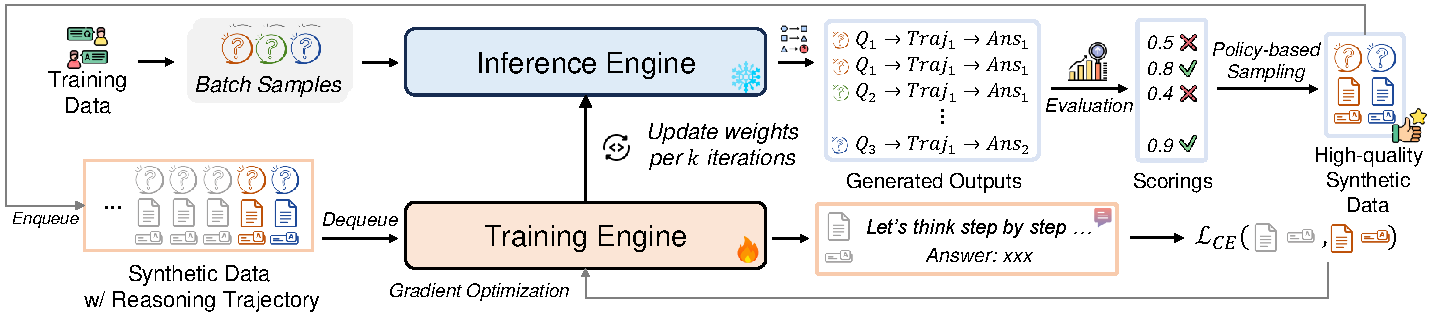
\includegraphics[width=\textwidth]{./figures/Mygo.pdf}
    \caption{The Proposed Minimalist Policy Gradient Optimization Framework.}
    \label{Mygo}
    % \vspace{-0.5em}
\end{figure*}

\subsection{Reinforcement Learning Setting}
% We implement our RAG agent in a conversation format. 
% A conversation (chat) is defined as a sequence of agent-environment interactions $(e_0, a_0, e_1, a_1, \dots, e_T, a_T )$, where $e_t$ is the environment message at time $t$, $a_t$ is agent's action at time step $t$, and $T$ is the maximum step.
% Note that $e_0$ includes a question and necessary prompts.
% We define chat state $s_t$ to be the chat history until $e_t$, i.e., $s_t = (e_0, a_0, e_1, a_1, \dots, e_t)$.
% A trajectory is $\tau = (s_0, a_0, \dots, s_t, a_t, \dots s_T, a_T)$.
% This is a Markov Decision Process.
% We denote trajectory's reward as $r(\tau)\in \R$, which is bounded by $M$.
% In our scenario, we do not have an immediate reward for each $a_t$; only trajectory-level reward is available.
Our RAG agent is implemented within a conversational framework.
A conversation is modeled as a finite sequence of interactions between the environment and the agent, denoted as $(e_0, a_0, e_1, a_1, \dots, e_T, a_T)$.
The initial environment message $e_0$ comprises the user's question and any necessary system prompts.
For each turn $t \in [0, T]$, $a_t$ is the agent's action, and $e_{t+1}$ is the subsequent environment message.
We define the state $s_t$ at turn $t$ as the history of all preceding interactions, $s_t = (e_0, a_0, e_1, a_1, \dots, a_{t-1}, e_t)$.
% A trajectory $\tau$ is the sequence of states and actions $\tau = (s_0, a_0, s_1, a_1, \dots, s_T, a_T)$. 
Then, a trajectory $\tau = (s_0, a_0, s_1, a_1, \dots, s_T, a_T)$ to the final answer of the question can be denoted as the sequence of states and actions in each step. 
%By defining the state as the complete history, the 
This formulation adheres to a Markov Decision Process (MDP).
Since the golden reasoning path to the ground truth answer is not available in real-world scenarios and most datasets,
 we do not have supervision signals for each action $a_t$ to conduct supervised finetuning.
The only supervision signal available to estimate the reward $r(\tau) \in \mathbb{R}$ for the entire trajectory $\tau$ is the final answer, which naturally corresponds to the terminal reward in an RL setting.

% Each trajectory $\tau$ is associated with a scalar reward $r(\tau) \in \mathbb{R}$, which is assume to be bounded by $M$.
% In our QA setting, only trajectory-level reward is available, i.e., no reward for intermediate actions.

% We denote the agent parametrized by $\theta$ as $\pi_\theta$.
% RL's learning objective is to maximize the expected reward $\mathcal{J}(\theta) = \E [ r(\tau)]$.
% If we can sample from $\pi_\theta$ and $\pi_\theta$ is differentiable, we can estimate $\mathcal{J}$ via Monte Carlo sampling and update $\theta$ by policy gradient~\cite{williams1992simple}:
% \begin{equation}
% \label{eq_vpo}
%     \nabla_\theta \mathcal{J}(\theta) = \underset{\tau \sim \pi_{\theta}}{\mathbb{E}}
%     \left[ r(\tau) \sum_{t=0}^T \nabla_\theta \log \pi_\theta (a_t | s_t)   \right] \;.
% \end{equation}

% The agent's policy $\pi_\theta$ is parameterized by $\theta$. 
We consider a policy-based method - the RAG agent adopts a policy $\pi_\theta$ to generate reasoning trajectories, where the parameters $\theta$ are optimized using RL techniques.
The objective of the RL is to find  the best policy that maximizes the expected cumulative reward:
\begin{equation}
\label{eq_obj}
     \mathcal{J}(\theta) = \mathbb{E}_{\tau \sim \pi_{\theta}} [r(\tau)] \; ,
\end{equation}
If trajectories sampled from $\pi_\theta$ are differentiable w.r.t. $\theta$, the gradient of the optimization objective can be estimated using the Vanilla Policy Gradient (VPO)~\citep{williams1992simple}:
\begin{equation}
\label{eq_vpo} % Ensure this label is unique in your document
\nabla_\theta \mathcal{J}(\theta) = \underset{\tau \sim \pi_{\theta}}{\mathbb{E}}
\left[ r(\tau) \sum_{t=0}^T \nabla_\theta \log \pi_\theta (a_t | s_t) \right] \;.
\end{equation}

% Since we are working on LLM agents, the likelihood can be further elaborated with token likelihood:
% \begin{equation}
% \label{eq_7}
%     \log \pi_\theta (a_t | s_t) = \sum_i \log \pi_\theta (o_i | o_{<i}) \;,
% \end{equation}
% where $o_i$ denotes the $i$-th token in $a_t$ and $o_{<i}$ denotes all tokens before $o_i$.
% Plugging Eq.~(\ref{eq_7}) into Eq.~(\ref{eq_6}), we have the gradient equivalent to token-level cross entropy up to constant
% \begin{equation}
% \label{eq_8}
%     \nabla_\theta \mathcal{J}(\theta) = \underset{\tau \sim \pi_{\theta_k}}{\mathbb{E}}
%     \left[ r(\tau) \sum_{t=0}^T \nabla_\theta \mathds{1}(o_i) \log \pi_\theta (o_i | o_{<i})
%     \right] \;,
% \end{equation}
% where $\mathds{1}(o_i)$ is a characteristic function indicating whether $o_i$ is an action token (1 for true 0 for false).

\subsection{Reinforcement Learning for LLMs}

% Traditional RL methods argue that though Vanilla Policy Gradient (VPO, Eq.~\ref{eq_vpo}) is unbiased, its variance could be large.
% Many methods~\cite{schulman2015trust, schulman2017proximal} attempt to stabilize variance by replacing the reward with Generalized Advantage Estimation~\cite{schulman2016high}.
% RL methods~\cite{schulman2017proximal, rafailov2023direct} have been widely applied in LLMs for alignment.
% Recently, GRPO~\cite{shao2024deepseekmath} proposes to simplify PPO~\cite{schulman2017proximal}'s value estimation with statistical estimation, which effectively reduces training cost and achieves comparable performance:
% \begin{equation}
% \label{eq_ppo}
%     \mathcal{J}(\theta) = \underset{\tau \sim \pi_{\theta_k}}{\mathbb{E}}
%     \left[ A(\tau) \sum_{t=0}^T
% \min \left(r_t, \;
% \text{clip}\left(r_t, 1-\epsilon, 1+\epsilon \right) \right)\right]
% - \beta \mathds{D}_{\text{KL}}(\pi_\theta || \pi_{\text{ref}})  \; ,
% \end{equation}
% where $\epsilon, \beta$ are hyper-parameters, $\pi_{\text{ref}}, \pi_{\theta_k}$ denotes the reference policy, the behavior policy, respectively; $r_t = \frac{\pi_\theta(a_t|s_t)}{\pi_{\theta_k}(a_t|s_t)}$ is the ratio of target policy and behavior policy, and $A(\tau)$ is trajectory advantage.
% In GRPO, the advantage function is estimated as $A(\tau)=\frac{r(\tau) - \Bar{r}}{\text{std}(r)}$, where $\Bar{r}, \text{std}(r)$ is mean and standard deviation of $r(\tau)$ within the same sampling group, respectively.

Even though the VPO (Eq.~\ref{eq_vpo}) estimator is unbiased,
it often exhibits high gradient variance, which potentially renders the training process unstable.
% Consequently, many attempts have been made to reduce the variance, with 
To address this issue, many previous approaches \cite{schulman2015trust, schulman2017proximal} propose to replace the raw trajectory reward $r(\tau)$ with the Generalized Advantage Estimation (GAE) \citep{schulman2016high}.
These RL techniques, particularly Proximal Policy Optimization (PPO)~\cite{schulman2017proximal} and its variants, have been successfully applied in the post-training process for LLM~\citep{ouyang2022training, rafailov2023direct}.
Recently, Group Relative Policy Optimization~(GRPO) \citep{shao2024deepseekmath} has been introduced as a simplified alternative to PPO, reducing the training costs while maintaining comparable performance.
The objective function of PPO and GRPO, as adapted for our QA context, can be written as follows:
\begin{equation}
\label{eq_ppo}
\begin{aligned}
    \mathcal{J}(\theta) = &\underset{\tau \sim \pi_{\theta_k}}{\mathbb{E}}
    \left[ A(\tau) \sum_{t=0}^T
\min \left(\mathbf{r}_t, \;
\text{clip}\left(\mathbf{r}_t, 1-\epsilon, 1+\epsilon \right) \right)\right]
\\& \hspace*{\fill} - \beta \mathds{D}_{\text{KL}}(\pi_\theta || \pi_{\text{ref}})  \; ,
\end{aligned}
\end{equation}
where $\epsilon, \beta$ are hyperparameters; $\pi_{\text{ref}}, \pi_{\theta_k}$ denote the reference policy and the behavior policy, respectively; 
$\mathbf{r}_t = \frac{\pi_\theta(a_t|s_t)}{\pi_{\theta_k}(a_t|s_t)}$ is the importance sampling rescaling factor; and $A(\tau)$ is the advantage of applying trajectory $\tau$.
Specifically, in PPO, the advantage function $A(\tau)$ is estimated by $r(\tau) - V(\tau)$, relying on a learnable value function $V(\tau)$.
In GRPO, $A(\tau)$ is instead estimated by $\frac{r(\tau) - \Bar{r}}{\text{std}(r)}$, where $\Bar{r}$ and $\text{std}(r)$ are the mean and standard deviation of $r(\tau)$ for each $\tau$ obtained from the same sampling group, respectively. 
% within the same sampling group, respectively.

% \subsection{Drawbacks of PPO-Style Objective}

% These PPO-style objective has two features.
% It constraints $\pi_\theta / \pi_{\theta_k}$ and constraints the gradient rescaling by replacing $r(\tau)$ with the advantage function.
% All these features cope with numerical instability due to non-stationary data distribution.
% Although applying importance sampling rescaling $\mathbf{r}_t$ and 
% All these features cope with numerical instability due to non-stationary data distribution.
% They have two drawbacks: hyper-parameter sensitivity and training inefficiency.
% Hyper-parameter refer to the fact that the boundary hyper-parameter $\epsilon$ controls the degree of how $\pi_\theta$ could change.
% A big $\epsilon$ lead to numerical instability and a small $\epsilon$ will disable the loss from many training examples and lead to training inefficiency.
% On the other hand, the standardization of reward in GRPO might lead to training inefficient.
% If the reward in one group is already high, GRPO will assign a relatively small scale to these trajectories.
% We argue that trajectories with high absolute value is important \cite{liu2024decade} and should not be discarded.
% The key feature of PPO-style optimization objectives lies in in the application of gradient rescaling for different data samples, which is primarily achieved by importance sampling and the clipping mechanism. However, the non-stationary nature of data distribution can make LLMs sensitive to hyperparameter selection.  For example, the boundary hyperparameter $\epsilon$ ich $\pi_\theta$ can change. A large $\epsilon$ can make the training process unstable, while a small $\epsilon$ may ignore the loss from a considerable amount othereby reducing the training efficiency. On the other hand, the standardization of reward in GRPO might lead to training inefficient. If the reward in one group is already high, GRPO will assign a relatively small scale to these trajectories. We argue that trajectories with high absolute value is important \cite{liu2024decade} and should not be discarded.



\subsection{MyGO}
% \subsection{\underline{M}inimalist Polic\underline{y} \underline{G}radient \underline{O}ptimization}
\label{sec:mygo}

% Compared with traditional RL scenarios \cite{openai2016gym} which are extremely stochastic, LLMs are more stable and reasonable, i.e., they rarely output nonsense words.
% Compared with traditional RL in robot control and video games \cite{openai2016gym} which are relatively stochastic, RL with LLMs show 3 properties: fast simulation, deterministic environment, and trajectory-level reward \cite{li2024remax}.
% We argue that some of the commonly adopted components like KL penalty, importance sampling clipping, are not decisive in the LLM post-training.
% We need new algorithm to accommodate the new setting.
% This raises an important research question, ``\textit{how does vanilla policy gradient work for LLMs?}''
% A key observation is that maximizing a trajectory's likelihood is equivalent to maximizing standard language modeling likelihood, Eq.~(\ref{eq_8}), which is widely used on continue pre-training~\cite{radford2018improving} and supervised fine-tuning~\cite{ouyang2022training}.
% Many previous works try to simplify RL algorithm for LLMs \cite{li2024remax, dongraft, shao2024deepseekmath}.

% Instead of using reward or GAE to scale gradients, we propose to filter trajectories and fix their reward to $1$, which leads to our methodology - \textbf{M}inimalist polic\textbf{y} \textbf{G}radient \textbf{O}ptimization (\textbf{MyGO}).
% Inspired by recent progress in filtering data in RL \cite{muennighoff2025s1, yu2025dapo}, we justify the power of data selection with mathematical reasoning.

% We propose \textbf{M}inimalist polic\textbf{y} \textbf{G}radient \textbf{O}ptimization (\textbf{MyGO}).
% MyGO consists of two steps, collecting data and optimization.
% MyGO directly sample from the optimal policy and update current policy via MLE.
% The motivation of MyGO is that we found a warm-up-ed agent has acceptable success rate and the fact of LLM fast simulation and the cost of sampling is cheap.
% Then \textit{why not directly sample from the optimal distribution and train data with MLE?}
% MyGO is designed for LLM setting:
% \begin{itemize}
%     \item fast simulation: sampling is cheap
%     \item deterministic environment: no state transition
%     \item trajectory-level: agent reward is simple, either pass or fail or softened version of them.
% \end{itemize}

Despite its wide adoption, a PPO-style objective has two shortcomings: hyperparameter sensitivity and training inefficiency.
The $\epsilon$ hyperparameter is highly sensitive - a small $\epsilon$ may ignore most available trajectories during training, leading to training inefficiency; while a large $\epsilon$ might lose control over the importance sampling scale, resulting in a less stable training process.
The advantage estimation renormalizes the original rewards relative to either the value functions or the group average, 
which weakens the supervision signals from trajectories with large rewards that are helpful for training~\cite{liu2024decade}.
It is worth mentioning that \emph{training inefficiency and instability are significant challenges when training LLMs, which is both computationally expensive and time-consuming.}
On the other hand, compared with previous RL scenarios in robot control and video games~\cite{openai2016gym}, the LLM setting poses a new characteristic: fast simulation, deterministic environment, and trajectory-level reward~\cite{li2024remax}.
In this scenario, \emph{sampling desired trajectories from the environment is relatively more efficient.} 

% Therefore, New RL algorithms are thus required to cope with the LLM's characteristics. 

To this end, we propose our new RL algorithm, \textbf{MyGO}: \textbf{M}inimalist Polic\textbf{y} \textbf{G}radient \textbf{O}ptimization, which shifts the burden from model training to trajectory sampling,
in which we can fully leverage the fast and relatively inexpensive simulation of LLMs~\cite{kwon2023efficient, zheng2024sglang}. 
% and relative cheap.
% Putting more resource in sampling is an acceptable tradeoff.
% We want to disentangle the training and sampling to simplify the complexity of previous methods, which allows for a more stable training.
Unlike previous methods, MyGO disentangles the RL training process into two phases: sampling and training.
During sampling, MyGO directly samples trajectories from the asymptotically optimal distribution and consequently allows the use of Maximum Likelihood Estimation (MLE) to optimize the policy function.
Notably, optimizing a model via MLE is simple, stable, and well established as a regular training technique widely used in unsupervised pre-training~\cite{radford2018improving} and supervised fine-tuning~\cite{ouyang2022training}.

% From our observation, we can sample a successful agent trajectory from a prompted or warmuped LLM with acceptable cost.
% Sampling from the optimal distribution is sampling from a stationary distribution.
% All the devil comes from the non-stationary distribution in RL.

\paragraph{Sampling}
\renewcommand{\cJ}{\mathcal{J}}
% We will illustrate how to sample from the optimal distribution.
% consider the learning object with entropy regularization $\mathcal{J}' = \E[r(\tau)] + \alpha \mathbf{H}(\pi)$,
% where $\alpha$ is the temperature parameter and $\mathbf{H}$ is the distribution entropy.
% To guide our sampling towards high-reward trajectories, w
We first characterize the target optimal distribution $\pi^*$.
Alternative to the original objective $\mathcal{J}$, we consider the expected reward with entropy regularization $\mathcal{J}' = \E[r(\tau)] + \alpha \mathbf{H}(\pi)$ with $\alpha \in \mathbb{R}^+$,
which, as a Boltzmann distribution \cite{ziebart2010modeling}, has a closed-form solution for the corresponding optimal policy, denoted as ${\pi'}^*$:
\begin{equation}
    \label{eq_boltzmann_optimal} % Ensure this label is unique
    \begin{aligned}
    {\pi'}^* (\tau) &= \frac{\exp (r(\tau)/\alpha)}{Z(\alpha)} \; ,  \\ \quad \text{where } Z(\alpha) &= \int_{\mathcal{T}} \exp (r(\tau')/\alpha) d\tau' \; ,
    \end{aligned}
\end{equation}
where $\alpha$ is the temperature and $Z(\alpha)$ is the partition function that normalizes the distribution over the space of all possible trajectories $\mathcal{T}$.
With a sufficiently small $\alpha \to 0$, we have $\cJ' \to \cJ$, thus ${\pi'}^* \to \pi^*$.
As $\alpha \to 0$,
${\pi'}^*$ becomes sharp and highly skewed,
concentrating its probability mass on trajectories yielding high rewards.
Therefore, given a sufficiently large threshold $K$ close to $\sup_{\tau \in \mathcal{T}} r(\tau)$,
sampling trajectories $\tau$ with $r(\tau) > K$ is asymptotically equivalent to sampling from the ${\pi'}^*$ and thus effectively approximating to sampling from the optimal policy ${\pi}^*$ of $\cJ$.

In practice, we relax the choice of $K$ by setting an update role of $K:= \max(K', (\bar{r}_n/(r_\text{sup} + 1))\cdot r_\text{sup})$, where $r_\text{sup}$ denotes $\sup_{\tau \in \mathcal{T}} r(\tau)$, $\bar{r}_n$ is the empirical average reward of a batch of $n$ sampled trajectories, and $K'$ is the previous threshold value which is initialized as a moderate value depending on the choice of dataset.
As the policy $\pi_\theta$ improved,  $K$ will be asymptotically close to $\sup_{\tau \in \mathcal{T}} r(\tau)$, thus making the sampling distribution close to ${\pi'}^*$.


We highlight that this approach is practically feasible for the reward landscapes for tasks of the LLM agent, which differ significantly from those in complex robotic control problems.
For LLM agents, trajectories frequently culminate in outcomes that are clearly classifiable as successful or unsuccessful.
Empirically, we observe that well-prompted LLMs can readily generate a significant proportion of such successful trajectories, which makes directly sampling from $\pi^*$ feasible.

% If the optimal policy $\pi^*$ is sharply concentrated on high-reward trajectories, then the selection of these high-reward trajectories effectively approximates sampling from $\pi^*$.







% the optimal policy $\pi^*$ is sharply concentrated on high-reward trajectories.


% We expect the objective $\mathcal{J}'$ to closely approximate to the original one (Eq.~\ref{eq_obj}), which require the $\alpha$ to be sufficiently small.
% % When $\alpha$ is small enough, the modified $J'$ almost has no different to original learning object $\mathcal{J}$.
% The introduction of entropy regularization allows us to have a closed-form for $\pi^*$, as a Boltzmann distribution \cite{ziebart2010modeling}:
% % \begin{equation}
% %     \pi^* (\tau) = \frac{\exp (r(\tau)/\alpha)}{\int \exp (r(\tau')/\alpha)d\tau}.
% % \end{equation}



% The central sampling problem then becomes generating trajectories that follow this optimal distribution $\pi^*$, with $\pi_\theta$ as a proposal.

% Compared with a complex robotic control problem, a LLM agent trajectory is either succeeded (high reward) or failed (low reward).
% As long as we can collect those high-valued trajectories, we are sampling from the optimal policy.
% From our observation, a prompted LLM already could generate considerable amount of high-reward trajectory, which makes the fact directly sampling from the optimal policy feasible.
% This is a key difference from previous RL scenarios.


Let $\pi^{>K}$ denote the distribution that consists of trajectories with $r > K$.
To clarify, we provide two propositions as follows, where the proofs can be found in Appendix~\ref{appendix_math_proof}:
\begin{restatable}{proposition}{klapprox}
\label{propos_1}
Given $\delta \in \R$, $\alpha \in \R$, there exists $K \in \R^+$ such that the following inequality holds:
\begin{equation*}
    \mathds{D}_{\text{KL}}(\pi^{>K} || \pi^*) < \delta \; 
\end{equation*}
\end{restatable}

\begin{restatable}{proposition}{varapprox}
\label{propos_2}
The following property holds when $\alpha$ approaches $0$:
    \begin{equation*}
        \underset{\pi^{>K}}{\Var[r]} \propto 1 / Z^{>K}(\alpha)^2 \; , \; Z^{>K}(\alpha) = \int^{\sup(r)}_K \exp(r/\alpha)dr
    \end{equation*}
\end{restatable}

Proposition~\ref{propos_1} states that if $K$ is sufficiently large, then $\pi^{>K}$ can always approximate $\pi^*$.
Proposition~\ref{propos_2} says the variance of $\pi^{>K}$ is small, considering that $Z$ is usually a large value.
These two propositions guarantee the proximity and stability of our proposed sampling strategy.


% MyGO has two ways to sample, MyGO-hard and MyGO-soft.
% MyGO-hard. In MyGO-hard, we use a hard threshold to filter trajectories.
% When the threshold is set to $k$; then any trajectory with reward less than $k$ will be filtered out.
% In MyGO-soft, we use rejection sampling \cite{liu2024statistical, neal2003slice} to sample from the current policy:
% First sample a trajectory, $\tau \sim \pi_\theta$;
% Then sample from uniform distribution $u \sim \mathbf{U}[0,1]$;
% Calculate criterion $c=\frac{r(\tau)}{M}$;
% If $u<c$, $\tau$ will be accepted.

% MyGO-hard is an approximation to optimal policy.
% Its proximity relies on threshold $k$.
% A bigger $k$ indicates higher proximity.
% MyGO-soft is an unbiased sampling method, but it might suffer from high variance.
% In our experiment, we found MyGO-hard is more stable.

\paragraph{Learning}
Once a sufficiently large dataset of optimal trajectories $\mathcal{D}$ has been collected, the optimization of policy $\pi_\theta$ can be simplified to maximizing the log-likelihood $\mathcal{L}$ of these trajectories.
The learning process can be conducted in an online or an offline manner.
This yields the following MLE gradient:
\begin{align}
% \vspace{-1em}
\label{eq_8}
    \nabla_\theta \mathcal{L} &=\frac{1}{|\mathcal{D}|}\sum_{\tau_i \in \mathcal{D}} \nabla_\theta \log \pi_\theta (\tau_i) \notag \\
    &= \frac{1}{|\mathcal{D}|}\sum_{\tau_i \in \mathcal{D}}
      \sum_{j=0}^{|\tau_i|} \nabla_\theta \mathds{1}(o_j^i) \log \pi_\theta (o_j^i | o_{<j}^i) \; ,
\end{align}
% \vspace{-1em}
where $o_j^i$ denotes the $j$-th token from $\tau_i$ and $o_{<j}^i$ denotes the sequence of tokens preceding $o_j$, $\mathds{1}(o_j)$ is a characteristic function indicating whether $o_j$ is a token from the agent.
The last equality holds because the action likelihood in the language setting could be further elaborated with token likelihood, i.e, $\log \pi_\theta (a_t | s_t) = \sum_j \log \pi_\theta (o_j | o_{<j})$.
% Compared with VPO, MLE (Eq.~\ref{eq_7}) drops the reward turn and use data from optimal policy instead of samling from current policy.
% Compared with PPO-style objective (Eq.~\ref{eq_ppo}), MLE has no advantage function, clip function, and importance sampling.

This MLE objective, Eq.~\ref{eq_8}, is equivalent to a standard cross-entropy loss function, widely used in both unsupervised pre-training \cite{radford2018improving} and supervised fine-tuning \cite{ouyang2022training} of language models.
Compared to PPO-style algorithms, Eq.~\ref{eq_ppo}, MLE does not incorporate an advantage function, policy ratio clipping, and importance sampling.
Similarly, unlike methods such as VPO, Eq.~\ref{eq_vpo}, MLE directly uses the curated data $\mathcal{D}$ for training and does not explicitly use reward values in the loss computation.
% We empirically found that MLE offer more stable training.
% We argue that the stability might come from less variance from data (all trajectories approximately i.i.d.), less variance on reward scaling (the reward range might be huge), the drop of importance sampling (the ratio might be unstable), and the log function.
% We leave the justification for future work.
% One the other hand, Eq.~\ref{eq_8} show the MLE is actually the cross-entropy loss function, which is widely used on unsupervised pre-training~\cite{radford2018improving} and supervised fine-tuning~\cite{ouyang2022training}.
We empirically observed that MLE leads to more stable training. We explain this increased stability by several factors: (i) the dataset $\mathcal{D}$ consists of trajectories sampled from a more stationary (approximated optimal) distribution, reducing variance compared to on-policy RL where the data distribution shifts rapidly; (ii) the direct use of a log-likelihood objective (cross-entropy) is often well-behaved and less sensitive to reward scaling issues that can affect RL algorithms; and (iii) the avoidance of importance sampling ratios, which can introduce instability if they become too large or small.
The implementation details are in Appendix~\ref{appendix_implementation_detail}.

Compared with previous works, like RAFT~\cite{dongraft} and STaR \cite{zelikman2022star}, which try to simplify RL in LLM post-training, we use a progressive threshold to select data.
More importantly, we provide a theoretical justification that elucidates why this approach, yet relatively simple, yields strong performance, offering novel insights into its efficacy.
% \subsection{Relation to Previous Work}
% RAFT \cite{dongraft}: sample the best trajectory from each group

% Best-K-of-N: \cite{nakano2021webgpt, cobbe2021training, touvron2023llama}


% \paragraph{Discussion}
% MyGO can be implemented in both offline or online manner



% \subsection{To Vanilla Policy Gradient Optimization to \textbf{M}inimalist Polic\textbf{y} \textbf{G}radient \textbf{O}ptimization (MyGO)}

% \textcolor{purple}{[Liheng: Draft; to be reconsidered]}


% Vanilla Policy Gradient with real value terminal reward can be written as:
% \begin{equation}
%     \begin{aligned}
%     \nabla_{\theta} J(\pi_{\theta}) &= \mathbb{E}_{\tau \sim \pi_{\theta}}\left[\sum_{t=0}^{T} \nabla_{\theta} \log \pi_{\theta}(a_t | s_t) A^{\pi_{\theta}}(s_t, a_t)\right] \\
%     &= \mathbb{E}_{\tau \sim \pi_{\theta}}\left[r(\tau) \sum_{t=0}^{T} \nabla_{\theta} \log \pi_{\theta}(a_t | s_t) \right] \\
%     % &= \int_{\mathcal{T}} \left[\sum_{t=0}^{T} \nabla_{\theta} \log \pi_{\theta}(a_t | s_t) A^{\pi_{\theta}}(s_t, a_t)\right] p(\tau | \pi_{\theta}) d\tau \\
%     \end{aligned}
%     \label{eq:vpg_terminal}
% \end{equation}


% If we consider the reward $r(\tau) \in [0, C]$ for a $C > 0$; there exists a probability density function $C \cdot p(\tau) = r(\tau)$.







% \begin{equation}
%     \begin{aligned}
%     \nabla_{\theta} J(\pi_{\theta}) &= \mathbb{E}_{\tau \sim \pi_{\theta}}\left[C \cdot p(\tau) \sum_{t=0}^{T} \nabla_{\theta} \log \pi_{\theta}(a_t | s_t) \right] \\
%     \end{aligned}
% \end{equation}